\documentclass[a4paper,11pt]{article}
\usepackage[utf8]{inputenc}\usepackage[T1]{fontenc}
\usepackage[english]{babel}\usepackage{lmodern}\usepackage{microtype}
\usepackage{amsmath,amssymb}\usepackage{geometry}
\geometry{a4paper,left=2.2cm,right=2.2cm,top=2.0cm,bottom=2.0cm}
\usepackage{booktabs,array}\usepackage{xcolor}
\definecolor{bokug}{RGB}{0,135,60}\usepackage{tikz}
\usetikzlibrary{arrows.meta,calc}
\usepackage{fancyhdr}\pagestyle{fancy}
\renewcommand{\headrulewidth}{0.4pt}
\usepackage{enumitem}\setlength{\parindent}{0pt}\setlength{\parskip}{4pt}

\begin{document}
\fancyhead[L]{\small VU Mechanik – LAWI 100515 (PI)}\fancyhead[R]{\small SS 2026}\fancyfoot[C]{\thepage}
\begin{center}{\large\bfseries\color{bokug}University of Natural Resources and Life Sciences, Vienna (BOKU)}\\[2pt]{\large\bfseries VU Mechanik – LAWI 100515 (PI)}\\[4pt]Exam \textbf{Group A} \hfill Date: 26.06.2026\\[2pt]\rule{\linewidth}{0.4pt}\end{center}

\begin{center}\textbf{\large Model solution}\end{center}
\begin{center}
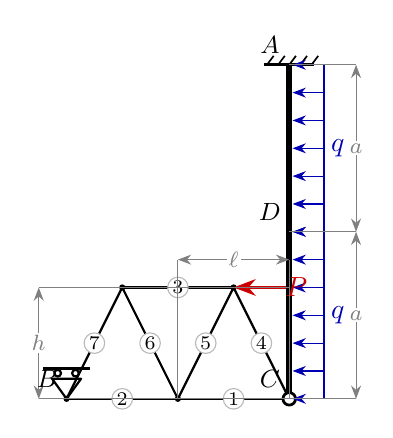
\begin{tikzpicture}[scale=0.707,>=Stealth,line join=round]
  \coordinate (P0) at (0.000,0.000);
  \coordinate (P1) at (0.000,-3.000);
  \coordinate (P2) at (0.000,-6.000);
  \coordinate (TO1) at (-2.000,-6.000);
  \coordinate (TO2) at (-4.000,-6.000);
  \coordinate (TU0) at (-1.000,-4.000);
  \coordinate (TU1) at (-3.000,-4.000);
  \draw[thick] (P2) -- (TO1);
  \draw[thick] (TO1) -- (TO2);
  \draw[thick] (TU0) -- (TU1);
  \draw[thick] (P2) -- (TU0);
  \draw[thick] (TU0) -- (TO1);
  \draw[thick] (TO1) -- (TU1);
  \draw[thick] (TU1) -- (TO2);
  \draw[line width=2.2pt] (P0) -- (P1);
  \draw[line width=2.2pt] (P1) -- (P2);
  \fill (TO1) circle (1.6pt);
  \fill (TO2) circle (1.6pt);
  \fill (TU0) circle (1.6pt);
  \fill (TU1) circle (1.6pt);
  \draw[fill=white,line width=1pt] (P2) circle (3.2pt);
  \draw[line width=1.1pt] (0.450,0.000) -- (-0.450,0.000);
  \draw[line width=0.6pt] (0.400,0.000) -- (0.520,0.160);
  \draw[line width=0.6pt] (0.200,0.000) -- (0.320,0.160);
  \draw[line width=0.6pt] (0.000,0.000) -- (0.120,0.160);
  \draw[line width=0.6pt] (-0.200,0.000) -- (-0.080,0.160);
  \draw[line width=0.6pt] (-0.400,0.000) -- (-0.280,0.160);
  \draw[thick] (-4.000,-6.000) -- (-3.740,-5.640) -- (-4.260,-5.640) -- cycle;
  \draw[thick] (-3.840,-5.540) circle (0.06) (-4.160,-5.540) circle (0.06);
  \draw[line width=1pt] (-3.580,-5.460) -- (-4.420,-5.460);
  \node[circle,fill=white,draw=gray!55,inner sep=0.5pt,font=\scriptsize] at (-1.000,-6.000) {1};
  \node[circle,fill=white,draw=gray!55,inner sep=0.5pt,font=\scriptsize] at (-3.000,-6.000) {2};
  \node[circle,fill=white,draw=gray!55,inner sep=0.5pt,font=\scriptsize] at (-2.000,-4.000) {3};
  \node[circle,fill=white,draw=gray!55,inner sep=0.5pt,font=\scriptsize] at (-0.500,-5.000) {4};
  \node[circle,fill=white,draw=gray!55,inner sep=0.5pt,font=\scriptsize] at (-1.500,-5.000) {5};
  \node[circle,fill=white,draw=gray!55,inner sep=0.5pt,font=\scriptsize] at (-2.500,-5.000) {6};
  \node[circle,fill=white,draw=gray!55,inner sep=0.5pt,font=\scriptsize] at (-3.500,-5.000) {7};
  \draw[->,blue!70!black] (0.620,0.000) -- (0.060,0.000);
  \draw[->,blue!70!black] (0.620,-0.500) -- (0.060,-0.500);
  \draw[->,blue!70!black] (0.620,-1.000) -- (0.060,-1.000);
  \draw[->,blue!70!black] (0.620,-1.500) -- (0.060,-1.500);
  \draw[->,blue!70!black] (0.620,-2.000) -- (0.060,-2.000);
  \draw[->,blue!70!black] (0.620,-2.500) -- (0.060,-2.500);
  \draw[->,blue!70!black] (0.620,-3.000) -- (0.060,-3.000);
  \draw[blue!70!black,thick] (0.620,0.000) -- (0.620,-3.000);
  \node[blue!70!black] at (0.870,-1.500) {$q$};
  \draw[->,blue!70!black] (0.620,-3.000) -- (0.060,-3.000);
  \draw[->,blue!70!black] (0.620,-3.500) -- (0.060,-3.500);
  \draw[->,blue!70!black] (0.620,-4.000) -- (0.060,-4.000);
  \draw[->,blue!70!black] (0.620,-4.500) -- (0.060,-4.500);
  \draw[->,blue!70!black] (0.620,-5.000) -- (0.060,-5.000);
  \draw[->,blue!70!black] (0.620,-5.500) -- (0.060,-5.500);
  \draw[->,blue!70!black] (0.620,-6.000) -- (0.060,-6.000);
  \draw[blue!70!black,thick] (0.620,-3.000) -- (0.620,-6.000);
  \node[blue!70!black] at (0.870,-4.500) {$q$};
  \draw[->,red!80!black,line width=1.1pt] (-0.050,-4.000) -- (-1.000,-4.000);
  \node[red!80!black] at (0.130,-4.000) {$P$};
  \draw[thin,gray] (0.000,0.000) -- (1.200,0.000);
  \draw[thin,gray] (0.000,-3.000) -- (1.200,-3.000);
  \draw[<->,gray] (1.200,0.000) -- (1.200,-3.000) node[midway,fill=white,inner sep=0.8pt,font=\footnotesize]{$a$};
  \draw[thin,gray] (0.000,-3.000) -- (1.200,-3.000);
  \draw[thin,gray] (0.000,-6.000) -- (1.200,-6.000);
  \draw[<->,gray] (1.200,-3.000) -- (1.200,-6.000) node[midway,fill=white,inner sep=0.8pt,font=\footnotesize]{$a$};
  \draw[thin,gray] (0.000,-6.000) -- (0.000,-3.500);
  \draw[thin,gray] (-2.000,-6.000) -- (-2.000,-3.500);
  \draw[<->,gray] (0.000,-3.500) -- (-2.000,-3.500) node[midway,fill=white,inner sep=0.8pt,font=\footnotesize]{$\ell$};
  \draw[thin,gray] (0.000,-6.000) -- (-4.500,-6.000);
  \draw[thin,gray] (0.000,-4.000) -- (-4.500,-4.000);
  \draw[<->,gray] (-4.500,-6.000) -- (-4.500,-4.000) node[midway,fill=white,inner sep=0.8pt,font=\footnotesize]{$h$};
  \node[font=\small] at (0.000,0.000) [xshift=-7pt,yshift=7pt] {$A$};
  \node[font=\small] at (0.000,-3.000) [xshift=-7pt,yshift=7pt] {$D$};
  \node[font=\small] at (0.000,-6.000) [xshift=-7pt,yshift=7pt] {$C$};
  \node[font=\small] at (-4.000,-6.000) [xshift=-7pt,yshift=7pt] {$B$};
\end{tikzpicture}
\end{center}
\par\medskip\textbf{1.\ Static determinacy}\par Counting criterion $n=3k-(a+z)$ (bodies $k$, reactions $a$, interaction forces $z$):
\[ n=3k-(a+z)=3\cdot2-(4+2)=0\ \Rightarrow\ \text{statically determinate} \]
\par\medskip\textbf{2.\ Support reactions and hinge forces}\par
$A:\ R_x=50,\ R_y=-10,\ M=210$\quad $B:\ R_x=0,\ R_y=10$\par $C:\ H_x=-20,\ H_y=10$
\par\medskip\textbf{3.\ Truss member forces}\par
\begin{center}\renewcommand{\arraystretch}{1.1}\begin{tabular}{c r l}
\toprule
Member & Force $S$ [kN] & Type \\
\midrule
  1 & 15 & tension \\
  2 & 5 & tension \\
  3 & -10 & compression \\
  4 & 11.18 & tension \\
  5 & -11.18 & compression \\
  6 & 11.18 & tension \\
  7 & -11.18 & compression \\
\bottomrule
\end{tabular}\end{center}
\begin{center}
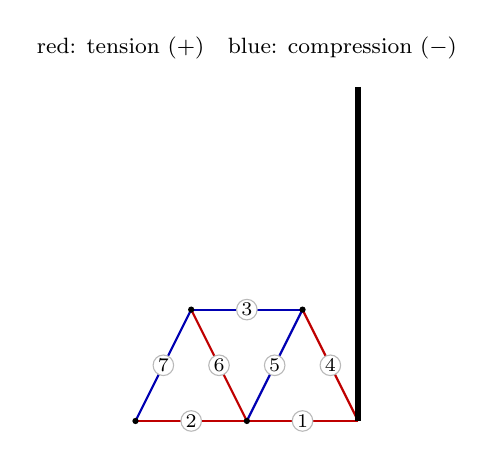
\begin{tikzpicture}[scale=0.707,>=Stealth,line join=round]
  \coordinate (P0) at (0.000,0.000);
  \coordinate (P1) at (0.000,-3.000);
  \coordinate (P2) at (0.000,-6.000);
  \coordinate (TO1) at (-2.000,-6.000);
  \coordinate (TO2) at (-4.000,-6.000);
  \coordinate (TU0) at (-1.000,-4.000);
  \coordinate (TU1) at (-3.000,-4.000);
  \draw[thick,red!75!black] (P2) -- (TO1);
  \draw[thick,red!75!black] (TO1) -- (TO2);
  \draw[thick,blue!70!black] (TU0) -- (TU1);
  \draw[thick,red!75!black] (P2) -- (TU0);
  \draw[thick,blue!70!black] (TU0) -- (TO1);
  \draw[thick,red!75!black] (TO1) -- (TU1);
  \draw[thick,blue!70!black] (TU1) -- (TO2);
  \draw[line width=2pt] (P0) -- (P1);
  \draw[line width=2pt] (P1) -- (P2);
  \fill (TO1) circle (1.6pt);
  \fill (TO2) circle (1.6pt);
  \fill (TU0) circle (1.6pt);
  \fill (TU1) circle (1.6pt);
  \node[circle,fill=white,draw=gray!55,inner sep=0.5pt,font=\scriptsize] at (-1.000,-6.000) {1};
  \node[circle,fill=white,draw=gray!55,inner sep=0.5pt,font=\scriptsize] at (-3.000,-6.000) {2};
  \node[circle,fill=white,draw=gray!55,inner sep=0.5pt,font=\scriptsize] at (-2.000,-4.000) {3};
  \node[circle,fill=white,draw=gray!55,inner sep=0.5pt,font=\scriptsize] at (-0.500,-5.000) {4};
  \node[circle,fill=white,draw=gray!55,inner sep=0.5pt,font=\scriptsize] at (-1.500,-5.000) {5};
  \node[circle,fill=white,draw=gray!55,inner sep=0.5pt,font=\scriptsize] at (-2.500,-5.000) {6};
  \node[circle,fill=white,draw=gray!55,inner sep=0.5pt,font=\scriptsize] at (-3.500,-5.000) {7};
  \node[font=\footnotesize] at (-2.00,0.70) {red: tension $(+)$\quad blue: compression $(-)$};
\end{tikzpicture}
\end{center}
\par\medskip\textbf{4.\ Section-force diagrams of the beams}\par
\begin{center}
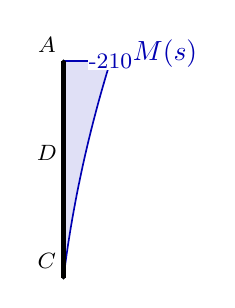
\begin{tikzpicture}[scale=0.459,line join=round]
  \filldraw[fill=blue!70!black!12,draw=blue!70!black,semithick] (1.300,0.000) -- (1.262,-0.125) -- (1.224,-0.250) -- (1.186,-0.375) -- (1.149,-0.500) -- (1.113,-0.625) -- (1.077,-0.750) -- (1.041,-0.875) -- (1.006,-1.000) -- (0.971,-1.125) -- (0.937,-1.250) -- (0.904,-1.375) -- (0.871,-1.500) -- (0.838,-1.625) -- (0.806,-1.750) -- (0.774,-1.875) -- (0.743,-2.000) -- (0.712,-2.125) -- (0.682,-2.250) -- (0.652,-2.375) -- (0.623,-2.500) -- (0.594,-2.625) -- (0.566,-2.750) -- (0.538,-2.875) -- (0.511,-3.000) -- (0.511,-3.000) -- (0.484,-3.125) -- (0.458,-3.250) -- (0.432,-3.375) -- (0.406,-3.500) -- (0.381,-3.625) -- (0.357,-3.750) -- (0.333,-3.875) -- (0.310,-4.000) -- (0.287,-4.125) -- (0.264,-4.250) -- (0.242,-4.375) -- (0.221,-4.500) -- (0.199,-4.625) -- (0.179,-4.750) -- (0.159,-4.875) -- (0.139,-5.000) -- (0.120,-5.125) -- (0.102,-5.250) -- (0.083,-5.375) -- (0.066,-5.500) -- (0.049,-5.625) -- (0.032,-5.750) -- (0.016,-5.875) -- (0.000,-6.000) -- (0.000,-6.000) -- (0.000,-5.875) -- (0.000,-5.750) -- (0.000,-5.625) -- (0.000,-5.500) -- (0.000,-5.375) -- (0.000,-5.250) -- (0.000,-5.125) -- (0.000,-5.000) -- (0.000,-4.875) -- (0.000,-4.750) -- (0.000,-4.625) -- (0.000,-4.500) -- (0.000,-4.375) -- (0.000,-4.250) -- (0.000,-4.125) -- (0.000,-4.000) -- (0.000,-3.875) -- (0.000,-3.750) -- (0.000,-3.625) -- (0.000,-3.500) -- (0.000,-3.375) -- (0.000,-3.250) -- (0.000,-3.125) -- (0.000,-3.000) -- (0.000,-3.000) -- (0.000,-2.875) -- (0.000,-2.750) -- (0.000,-2.625) -- (0.000,-2.500) -- (0.000,-2.375) -- (0.000,-2.250) -- (0.000,-2.125) -- (0.000,-2.000) -- (0.000,-1.875) -- (0.000,-1.750) -- (0.000,-1.625) -- (0.000,-1.500) -- (0.000,-1.375) -- (0.000,-1.250) -- (0.000,-1.125) -- (0.000,-1.000) -- (0.000,-0.875) -- (0.000,-0.750) -- (0.000,-0.625) -- (0.000,-0.500) -- (0.000,-0.375) -- (0.000,-0.250) -- (0.000,-0.125) -- (0.000,0.000) -- cycle;
  \draw[line width=1.6pt] (0.000,0.000) -- (0.000,-3.000) -- (0.000,-6.000);
  \node[blue!70!black,font=\footnotesize,fill=white,inner sep=0.5pt] at (1.300,0.000) {-210};
  \fill (0.000,0.000) circle (1.3pt);
  \node[font=\footnotesize] at (0.000,0.000) [xshift=-6pt,yshift=6pt] {$A$};
  \fill (0.000,-3.000) circle (1.3pt);
  \node[font=\footnotesize] at (0.000,-3.000) [xshift=-6pt,yshift=6pt] {$D$};
  \fill (0.000,-6.000) circle (1.3pt);
  \node[font=\footnotesize] at (0.000,-6.000) [xshift=-6pt,yshift=6pt] {$C$};
  \node[blue!70!black,right] at (1.65,0.20) {$M(s)$};
\end{tikzpicture}\\[5pt]
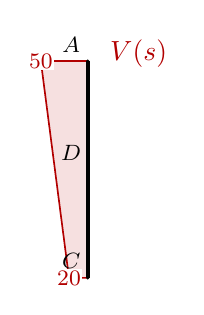
\begin{tikzpicture}[scale=0.459,line join=round]
  \filldraw[fill=red!70!black!12,draw=red!70!black,semithick] (-1.300,0.000) -- (-1.284,-0.125) -- (-1.268,-0.250) -- (-1.251,-0.375) -- (-1.235,-0.500) -- (-1.219,-0.625) -- (-1.203,-0.750) -- (-1.186,-0.875) -- (-1.170,-1.000) -- (-1.154,-1.125) -- (-1.138,-1.250) -- (-1.121,-1.375) -- (-1.105,-1.500) -- (-1.089,-1.625) -- (-1.073,-1.750) -- (-1.056,-1.875) -- (-1.040,-2.000) -- (-1.024,-2.125) -- (-1.008,-2.250) -- (-0.991,-2.375) -- (-0.975,-2.500) -- (-0.959,-2.625) -- (-0.943,-2.750) -- (-0.926,-2.875) -- (-0.910,-3.000) -- (-0.910,-3.000) -- (-0.894,-3.125) -- (-0.878,-3.250) -- (-0.861,-3.375) -- (-0.845,-3.500) -- (-0.829,-3.625) -- (-0.813,-3.750) -- (-0.796,-3.875) -- (-0.780,-4.000) -- (-0.764,-4.125) -- (-0.748,-4.250) -- (-0.731,-4.375) -- (-0.715,-4.500) -- (-0.699,-4.625) -- (-0.683,-4.750) -- (-0.666,-4.875) -- (-0.650,-5.000) -- (-0.634,-5.125) -- (-0.618,-5.250) -- (-0.601,-5.375) -- (-0.585,-5.500) -- (-0.569,-5.625) -- (-0.553,-5.750) -- (-0.536,-5.875) -- (-0.520,-6.000) -- (0.000,-6.000) -- (0.000,-5.875) -- (0.000,-5.750) -- (0.000,-5.625) -- (0.000,-5.500) -- (0.000,-5.375) -- (0.000,-5.250) -- (0.000,-5.125) -- (0.000,-5.000) -- (0.000,-4.875) -- (0.000,-4.750) -- (0.000,-4.625) -- (0.000,-4.500) -- (0.000,-4.375) -- (0.000,-4.250) -- (0.000,-4.125) -- (0.000,-4.000) -- (0.000,-3.875) -- (0.000,-3.750) -- (0.000,-3.625) -- (0.000,-3.500) -- (0.000,-3.375) -- (0.000,-3.250) -- (0.000,-3.125) -- (0.000,-3.000) -- (0.000,-3.000) -- (0.000,-2.875) -- (0.000,-2.750) -- (0.000,-2.625) -- (0.000,-2.500) -- (0.000,-2.375) -- (0.000,-2.250) -- (0.000,-2.125) -- (0.000,-2.000) -- (0.000,-1.875) -- (0.000,-1.750) -- (0.000,-1.625) -- (0.000,-1.500) -- (0.000,-1.375) -- (0.000,-1.250) -- (0.000,-1.125) -- (0.000,-1.000) -- (0.000,-0.875) -- (0.000,-0.750) -- (0.000,-0.625) -- (0.000,-0.500) -- (0.000,-0.375) -- (0.000,-0.250) -- (0.000,-0.125) -- (0.000,0.000) -- cycle;
  \draw[line width=1.6pt] (0.000,0.000) -- (0.000,-3.000) -- (0.000,-6.000);
  \node[red!70!black,font=\footnotesize,fill=white,inner sep=0.5pt] at (-1.300,0.000) {50};
  \node[red!70!black,font=\footnotesize,fill=white,inner sep=0.5pt] at (-0.520,-6.000) {20};
  \fill (0.000,0.000) circle (1.3pt);
  \node[font=\footnotesize] at (0.000,0.000) [xshift=-6pt,yshift=6pt] {$A$};
  \fill (0.000,-3.000) circle (1.3pt);
  \node[font=\footnotesize] at (0.000,-3.000) [xshift=-6pt,yshift=6pt] {$D$};
  \fill (0.000,-6.000) circle (1.3pt);
  \node[font=\footnotesize] at (0.000,-6.000) [xshift=-6pt,yshift=6pt] {$C$};
  \node[red!70!black,right] at (0.35,0.20) {$V(s)$};
\end{tikzpicture}\\[5pt]
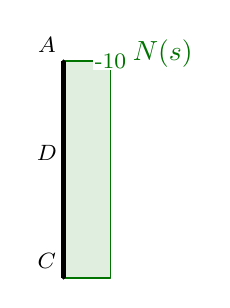
\begin{tikzpicture}[scale=0.459,line join=round]
  \filldraw[fill=green!45!black!12,draw=green!45!black,semithick] (1.300,0.000) -- (1.300,-0.125) -- (1.300,-0.250) -- (1.300,-0.375) -- (1.300,-0.500) -- (1.300,-0.625) -- (1.300,-0.750) -- (1.300,-0.875) -- (1.300,-1.000) -- (1.300,-1.125) -- (1.300,-1.250) -- (1.300,-1.375) -- (1.300,-1.500) -- (1.300,-1.625) -- (1.300,-1.750) -- (1.300,-1.875) -- (1.300,-2.000) -- (1.300,-2.125) -- (1.300,-2.250) -- (1.300,-2.375) -- (1.300,-2.500) -- (1.300,-2.625) -- (1.300,-2.750) -- (1.300,-2.875) -- (1.300,-3.000) -- (1.300,-3.000) -- (1.300,-3.125) -- (1.300,-3.250) -- (1.300,-3.375) -- (1.300,-3.500) -- (1.300,-3.625) -- (1.300,-3.750) -- (1.300,-3.875) -- (1.300,-4.000) -- (1.300,-4.125) -- (1.300,-4.250) -- (1.300,-4.375) -- (1.300,-4.500) -- (1.300,-4.625) -- (1.300,-4.750) -- (1.300,-4.875) -- (1.300,-5.000) -- (1.300,-5.125) -- (1.300,-5.250) -- (1.300,-5.375) -- (1.300,-5.500) -- (1.300,-5.625) -- (1.300,-5.750) -- (1.300,-5.875) -- (1.300,-6.000) -- (0.000,-6.000) -- (0.000,-5.875) -- (0.000,-5.750) -- (0.000,-5.625) -- (0.000,-5.500) -- (0.000,-5.375) -- (0.000,-5.250) -- (0.000,-5.125) -- (0.000,-5.000) -- (0.000,-4.875) -- (0.000,-4.750) -- (0.000,-4.625) -- (0.000,-4.500) -- (0.000,-4.375) -- (0.000,-4.250) -- (0.000,-4.125) -- (0.000,-4.000) -- (0.000,-3.875) -- (0.000,-3.750) -- (0.000,-3.625) -- (0.000,-3.500) -- (0.000,-3.375) -- (0.000,-3.250) -- (0.000,-3.125) -- (0.000,-3.000) -- (0.000,-3.000) -- (0.000,-2.875) -- (0.000,-2.750) -- (0.000,-2.625) -- (0.000,-2.500) -- (0.000,-2.375) -- (0.000,-2.250) -- (0.000,-2.125) -- (0.000,-2.000) -- (0.000,-1.875) -- (0.000,-1.750) -- (0.000,-1.625) -- (0.000,-1.500) -- (0.000,-1.375) -- (0.000,-1.250) -- (0.000,-1.125) -- (0.000,-1.000) -- (0.000,-0.875) -- (0.000,-0.750) -- (0.000,-0.625) -- (0.000,-0.500) -- (0.000,-0.375) -- (0.000,-0.250) -- (0.000,-0.125) -- (0.000,0.000) -- cycle;
  \draw[line width=1.6pt] (0.000,0.000) -- (0.000,-3.000) -- (0.000,-6.000);
  \node[green!45!black,font=\footnotesize,fill=white,inner sep=0.5pt] at (1.300,0.000) {-10};
  \fill (0.000,0.000) circle (1.3pt);
  \node[font=\footnotesize] at (0.000,0.000) [xshift=-6pt,yshift=6pt] {$A$};
  \fill (0.000,-3.000) circle (1.3pt);
  \node[font=\footnotesize] at (0.000,-3.000) [xshift=-6pt,yshift=6pt] {$D$};
  \fill (0.000,-6.000) circle (1.3pt);
  \node[font=\footnotesize] at (0.000,-6.000) [xshift=-6pt,yshift=6pt] {$C$};
  \node[green!45!black,right] at (1.65,0.20) {$N(s)$};
\end{tikzpicture}\\[10pt]
\end{center}
\end{document}